\documentclass{standalone}
\usepackage{tikz}
\usetikzlibrary{patterns, positioning}

\begin{document}
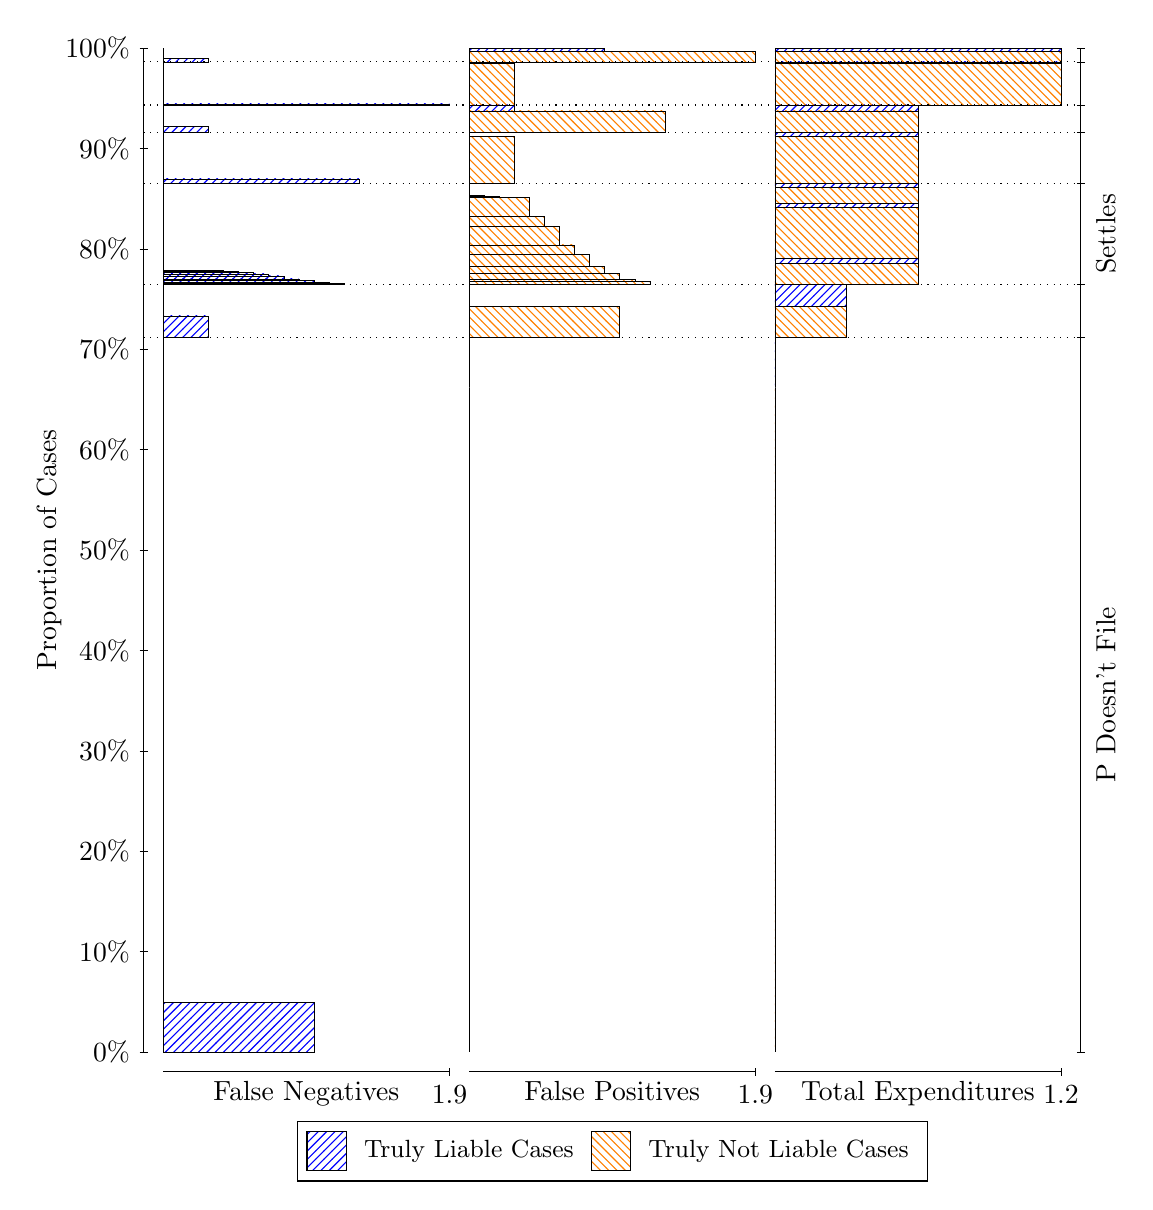
\begin{tikzpicture}
\draw[black, very thin] (1.5,1.75) -- (1.5,14.5);
\node[rotate=90, anchor=center] at (0.3, 8.125) {Proportion of Cases};
\draw[black, very thin] (1.45,1.75) -- (1.55,1.75);
\node[anchor=east] at (1.45, 1.75) {0\%};
\draw[black, very thin] (1.45,3.025) -- (1.55,3.025);
\node[anchor=east] at (1.45, 3.025) {10\%};
\draw[black, very thin] (1.45,4.3) -- (1.55,4.3);
\node[anchor=east] at (1.45, 4.3) {20\%};
\draw[black, very thin] (1.45,5.575) -- (1.55,5.575);
\node[anchor=east] at (1.45, 5.575) {30\%};
\draw[black, very thin] (1.45,6.85) -- (1.55,6.85);
\node[anchor=east] at (1.45, 6.85) {40\%};
\draw[black, very thin] (1.45,8.125) -- (1.55,8.125);
\node[anchor=east] at (1.45, 8.125) {50\%};
\draw[black, very thin] (1.45,9.4) -- (1.55,9.4);
\node[anchor=east] at (1.45, 9.4) {60\%};
\draw[black, very thin] (1.45,10.675) -- (1.55,10.675);
\node[anchor=east] at (1.45, 10.675) {70\%};
\draw[black, very thin] (1.45,11.95) -- (1.55,11.95);
\node[anchor=east] at (1.45, 11.95) {80\%};
\draw[black, very thin] (1.45,13.225) -- (1.55,13.225);
\node[anchor=east] at (1.45, 13.225) {90\%};
\draw[black, very thin] (1.45,14.5) -- (1.55,14.5);
\node[anchor=east] at (1.45, 14.5) {100\%};

\draw[black, very thin] (13.4,1.75) -- (13.4,14.5);
\draw[black, very thin] (13.35,1.75) -- (13.45,1.75);
\node[anchor=west] at (13.35, 1.75) {};
\draw[black, very thin] (13.35,10.824) -- (13.45,10.824);
\node[anchor=west] at (13.35, 10.824) {};
\draw[black, very thin] (13.35,11.498) -- (13.45,11.498);
\node[anchor=west] at (13.35, 11.498) {};
\draw[black, very thin] (13.35,12.783) -- (13.45,12.783);
\node[anchor=west] at (13.35, 12.783) {};
\draw[black, very thin] (13.35,13.431) -- (13.45,13.431);
\node[anchor=west] at (13.35, 13.431) {};
\draw[black, very thin] (13.35,13.777) -- (13.45,13.777);
\node[anchor=west] at (13.35, 13.777) {};
\draw[black, very thin] (13.35,14.325) -- (13.45,14.325);
\node[anchor=west] at (13.35, 14.325) {};
\draw[black, very thin] (13.35,14.5) -- (13.45,14.5);
\node[anchor=west] at (13.35, 14.5) {};

\draw[black, very thin, pattern color=blue, pattern=north east lines] (1.75,1.75) rectangle (3.6623,2.3837);
\draw[black, very thin, pattern color=orange, pattern=north west lines] (1.75,2.3837) rectangle (1.75,10.824);
\draw[black, very thin, pattern color=blue, pattern=north east lines] (1.75,10.824) rectangle (2.3237,11.099);
\draw[black, very thin, pattern color=orange, pattern=north west lines] (1.75,11.099) rectangle (1.75,11.498);
\draw[black, very thin, pattern color=blue, pattern=north east lines] (1.75,11.498) rectangle (4.0447,11.509);
\draw[black, very thin, pattern color=blue, pattern=north east lines] (1.75,11.509) rectangle (3.8535,11.52);
\draw[black, very thin, pattern color=blue, pattern=north east lines] (1.75,11.52) rectangle (3.6623,11.546);
\draw[black, very thin, pattern color=blue, pattern=north east lines] (1.75,11.546) rectangle (3.4711,11.554);
\draw[black, very thin, pattern color=blue, pattern=north east lines] (1.75,11.554) rectangle (3.4711,11.568);
\draw[black, very thin, pattern color=blue, pattern=north east lines] (1.75,11.568) rectangle (3.2798,11.607);
\draw[black, very thin, pattern color=blue, pattern=north east lines] (1.75,11.607) rectangle (3.0886,11.631);
\draw[black, very thin, pattern color=blue, pattern=north east lines] (1.75,11.631) rectangle (2.8974,11.654);
\draw[black, very thin, pattern color=blue, pattern=north east lines] (1.75,11.654) rectangle (2.7061,11.662);
\draw[black, very thin, pattern color=blue, pattern=north east lines] (1.75,11.662) rectangle (2.5149,11.673);
\draw[black, very thin, pattern color=orange, pattern=north west lines] (1.75,11.673) rectangle (1.75,12.783);
\draw[black, very thin, pattern color=blue, pattern=north east lines] (1.75,12.783) rectangle (4.236,12.838);
\draw[black, very thin, pattern color=orange, pattern=north west lines] (1.75,12.838) rectangle (1.75,13.431);
\draw[black, very thin, pattern color=blue, pattern=north east lines] (1.75,13.431) rectangle (2.3237,13.506);
\draw[black, very thin, pattern color=orange, pattern=north west lines] (1.75,13.506) rectangle (1.75,13.777);
\draw[black, very thin, pattern color=blue, pattern=north east lines] (1.75,13.777) rectangle (5.3833,13.791);
\draw[black, very thin, pattern color=orange, pattern=north west lines] (1.75,13.791) rectangle (1.75,14.325);
\draw[black, very thin, pattern color=blue, pattern=north east lines] (1.75,14.325) rectangle (2.3237,14.371);
\draw[black, very thin, pattern color=orange, pattern=north west lines] (1.75,14.371) rectangle (1.75,14.5);
\draw[black, very thin, pattern color=orange, pattern=north west lines] (5.6333,1.75) rectangle (5.6333,10.19);
\draw[black, very thin, pattern color=blue, pattern=north east lines] (5.6333,10.19) rectangle (5.6333,10.824);
\draw[black, very thin, pattern color=orange, pattern=north west lines] (5.6333,10.824) rectangle (7.5456,11.223);
\draw[black, very thin, pattern color=blue, pattern=north east lines] (5.6333,11.223) rectangle (5.6333,11.498);
\draw[black, very thin, pattern color=orange, pattern=north west lines] (5.6333,11.498) rectangle (7.9281,11.532);
\draw[black, very thin, pattern color=orange, pattern=north west lines] (5.6333,11.532) rectangle (7.7368,11.562);
\draw[black, very thin, pattern color=orange, pattern=north west lines] (5.6333,11.562) rectangle (7.5456,11.637);
\draw[black, very thin, pattern color=orange, pattern=north west lines] (5.6333,11.637) rectangle (7.3544,11.725);
\draw[black, very thin, pattern color=orange, pattern=north west lines] (5.6333,11.725) rectangle (7.1632,11.884);
\draw[black, very thin, pattern color=orange, pattern=north west lines] (5.6333,11.884) rectangle (6.9719,12);
\draw[black, very thin, pattern color=orange, pattern=north west lines] (5.6333,12) rectangle (6.7807,12.231);
\draw[black, very thin, pattern color=orange, pattern=north west lines] (5.6333,12.231) rectangle (6.5895,12.362);
\draw[black, very thin, pattern color=orange, pattern=north west lines] (5.6333,12.362) rectangle (6.3982,12.607);
\draw[black, very thin, pattern color=blue, pattern=north east lines] (5.6333,12.607) rectangle (6.0158,12.619);
\draw[black, very thin, pattern color=blue, pattern=north east lines] (5.6333,12.619) rectangle (5.8246,12.626);
\draw[black, very thin, pattern color=blue, pattern=north east lines] (5.6333,12.626) rectangle (5.6333,12.783);
\draw[black, very thin, pattern color=orange, pattern=north west lines] (5.6333,12.783) rectangle (6.207,13.376);
\draw[black, very thin, pattern color=blue, pattern=north east lines] (5.6333,13.376) rectangle (5.6333,13.431);
\draw[black, very thin, pattern color=orange, pattern=north west lines] (5.6333,13.431) rectangle (8.1193,13.702);
\draw[black, very thin, pattern color=blue, pattern=north east lines] (5.6333,13.702) rectangle (6.207,13.777);
\draw[black, very thin, pattern color=orange, pattern=north west lines] (5.6333,13.777) rectangle (6.207,14.311);
\draw[black, very thin, pattern color=blue, pattern=north east lines] (5.6333,14.311) rectangle (5.6333,14.325);
\draw[black, very thin, pattern color=orange, pattern=north west lines] (5.6333,14.325) rectangle (9.2667,14.454);
\draw[black, very thin, pattern color=blue, pattern=north east lines] (5.6333,14.454) rectangle (7.3544,14.5);
\draw[black, very thin, pattern color=orange, pattern=north west lines] (9.5167,1.75) rectangle (9.5167,10.19);
\draw[black, very thin, pattern color=blue, pattern=north east lines] (9.5167,10.19) rectangle (9.5167,10.824);
\draw[black, very thin, pattern color=orange, pattern=north west lines] (9.5167,10.824) rectangle (10.425,11.223);
\draw[black, very thin, pattern color=blue, pattern=north east lines] (9.5167,11.223) rectangle (10.425,11.498);
\draw[black, very thin, pattern color=orange, pattern=north west lines] (9.5167,11.498) rectangle (11.333,11.762);
\draw[black, very thin, pattern color=blue, pattern=north east lines] (9.5167,11.762) rectangle (11.333,11.83);
\draw[black, very thin, pattern color=orange, pattern=north west lines] (9.5167,11.83) rectangle (11.333,12.472);
\draw[black, very thin, pattern color=blue, pattern=north east lines] (9.5167,12.472) rectangle (11.333,12.529);
\draw[black, very thin, pattern color=orange, pattern=north west lines] (9.5167,12.529) rectangle (11.333,12.733);
\draw[black, very thin, pattern color=blue, pattern=north east lines] (9.5167,12.733) rectangle (11.333,12.783);
\draw[black, very thin, pattern color=orange, pattern=north west lines] (9.5167,12.783) rectangle (11.333,13.376);
\draw[black, very thin, pattern color=blue, pattern=north east lines] (9.5167,13.376) rectangle (11.333,13.431);
\draw[black, very thin, pattern color=orange, pattern=north west lines] (9.5167,13.431) rectangle (11.333,13.702);
\draw[black, very thin, pattern color=blue, pattern=north east lines] (9.5167,13.702) rectangle (11.333,13.777);
\draw[black, very thin, pattern color=orange, pattern=north west lines] (9.5167,13.777) rectangle (13.15,14.311);
\draw[black, very thin, pattern color=blue, pattern=north east lines] (9.5167,14.311) rectangle (13.15,14.325);
\draw[black, very thin, pattern color=orange, pattern=north west lines] (9.5167,14.325) rectangle (13.15,14.454);
\draw[black, very thin, pattern color=blue, pattern=north east lines] (9.5167,14.454) rectangle (13.15,14.5);
\draw[black, dotted] (1.5,10.824) -- (13.4,10.824);
\draw[black, dotted] (1.5,11.498) -- (13.4,11.498);
\draw[black, dotted] (1.5,12.783) -- (13.4,12.783);
\draw[black, dotted] (1.5,13.431) -- (13.4,13.431);
\draw[black, dotted] (1.5,13.777) -- (13.4,13.777);
\draw[black, dotted] (1.5,14.325) -- (13.4,14.325);
\draw[black, very thin] (1.75,1.5) -- (5.3833,1.5);
\node[anchor=north] at (3.5667, 1.5) {False Negatives};
\draw[black, very thin] (5.3833,1.45) -- (5.3833,1.55);
\node[anchor=north] at (5.3833, 1.45) {1.9};

\draw[black, very thin] (5.6333,1.5) -- (9.2667,1.5);
\node[anchor=north] at (7.45, 1.5) {False Positives};
\draw[black, very thin] (9.2667,1.45) -- (9.2667,1.55);
\node[anchor=north] at (9.2667, 1.45) {1.9};

\draw[black, very thin] (9.5167,1.5) -- (13.15,1.5);
\node[anchor=north] at (11.333, 1.5) {Total Expenditures};
\draw[black, very thin] (13.15,1.45) -- (13.15,1.55);
\node[anchor=north] at (13.15, 1.45) {1.2};

\node[black, centered, rotate=90] at (13.72, 6.287) {P Doesn't File};

\node[black, centered, rotate=90] at (13.72, 12.14) {Settles};





\draw (7.449999999999999,1.5) node[draw=none] (baseCoordinate) {};
\begin{scope}[align=center]
        \matrix[scale=0.5, draw=black, below=0.5cm of baseCoordinate, nodes={draw}, column sep=0.1cm]{
            \node[rectangle, draw, minimum width=0.5cm, minimum height=0.5cm, pattern=north east lines, pattern color=blue] {}; &
            \node[draw=none, font=\small] (B) {Truly Liable Cases}; &
            \node[rectangle, draw, minimum width=0.5cm, minimum height=0.5cm, pattern=north west lines, pattern color=orange] {}; &
            \node[draw=none, font=\small] (B) {Truly Not Liable Cases}; \\
            };
\end{scope}

\end{tikzpicture}
\end{document}